In this Section, the results of the implementation of the machine learning algorithms on the binary classification dataset are presented. For each machine learning algorithm, the first step is to find the most suitable size of the moving window $m$ between $2$ (features only for current day) and $100$ (size of the developed binary classification dataset). If applicable, for each value of $m$ the hyperparameters are optimized. The results are reported with suitable graphs and similar representations. Finally, for each machine learning algorithm, the performance on the test set is evaluated. The test performance is the final rating of each algorithm.\\

Besides the three machine learning algorithms described in the theory Section, here, the performance of a simple majority predictor is evaluated. The majority predictor is used as a reference for the performance of the other machine learning algorithms.

\subsection{Majority Predictor}
The majority predictor is a naive approach for solving the binary classfication problem. It constantly predicts the label that occurs most often in the training set. Fig.~\ref{fig:major_acc_vs_m} reports the training accuracy (on the whole training set) and the 10-fold CV accuracy for the majority predictor. As expected, both accuracies are the same and coincide with the \SI{53.95}{\percent} labels $1$ in the training set, see Fig.~\ref{fig:test}. There is also no dependence of the accuracy on the length $m$ of the moving window because the majority predictor depends only on the labels but not on the features of the examples in the training set.\\

Tab.~\ref{tab:major_conf_mat} reports the confusion matrix of the majority predictor on the test set. Clearly, the majority predictor predicts only the majority label $1$, an increasement of tomorrow's Bitcoin market price.  This explains also the sensitivity and specificity of the majority predictor in Tab.~\ref{tab:major_results}. The Table additionally reports the test accuracy of the majority predictor which is given by \SI{55.54}{\percent}. Again, this is simply the frequency of the label $1$ in the test set, see Fig.~\ref{fig:test}.

\begin{figure}[h!]
  \centering
  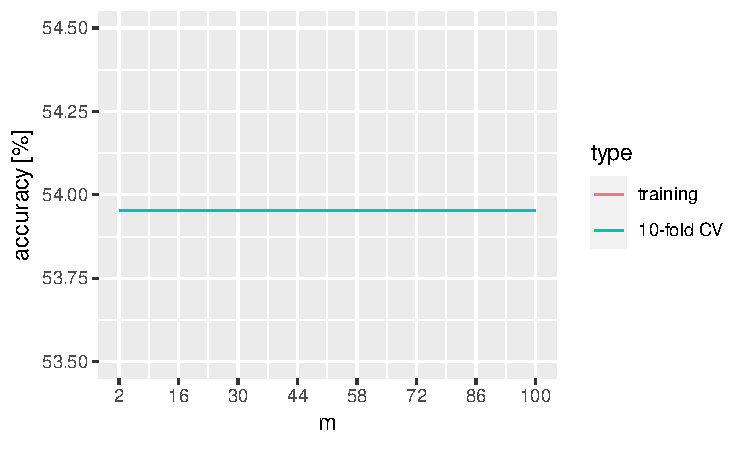
\includegraphics[width=0.8\textwidth]{major_acc_vs_m.pdf}
  \caption{Training and 10-fold CV accuracy of the majority predictor as a function of the length $m$ of the moving window.}
  \label{fig:major_acc_vs_m}
\end{figure}

\begin{table}[h!]
\centering
\begin{tabular}{c|c|c|c|c}
  \backslashbox{predicted}{true} & $0$ & $1$ \\
 \hline
 $0$ & $0$ & $0$ \\  
 \hline
 $1$ & $309$ & $386$    
\end{tabular}
 \caption{Confusion matrix of the majority predictor on the test set.}
 \label{tab:major_conf_mat}
\end{table}

\begin{table}[h!]
\centering
\begin{tabular}{c|c|c}
accuracy [\%] & sensitivity [\%] & specificity [\%] \\
   \hline
$55.54$ & $100.00$ & $0.00$
\end{tabular}
 \caption{Accuracy, sensitivity, and specificity of the majority predictor on the test set.}
 \label{tab:major_results}
\end{table}

\subsection{Logistic Regression}
A more sophisticated algorithm compared to the majority predictor is the logistic regression. Fig.~\ref{fig:log_acc_vs_m} shows the training and 10-fold CV accuracy for the logistic regression as a function of the moving window length $m$. The 10-fold CV accuracy of the logistic regression fit is maximized for a moving window length of $m=4$. The training accuracy increases significantly with $m$. The main reason for this is that an increase of $m$ is equivalent to the inclusion of more features. The model uses these features to \enquote{store} the training examples, which leads to comparably high training accuracies. However, the general performance of the logistic regression does not improve with increasing $m$ as can be verified by the slightly decreasing 10-fold CV accuracy.\\

Fig.~\ref{fig:log_roc} shows the so-called receiver operating characteristic (ROC) curve of the logistic regression fit. Recall that the logistic regression fit assigns a probability to all possible feature combinations that the label is $1$. Then, predictions are made by applying a probability threshold that depends, for which typically \SI{50}{\percent} is used. The ROC curve displays the sensitivity and specificity for all possible values of this threshold from \SI{0}{\percent} in the upper righthand corner to \SI{100}{\percent} in the lower lefthand corner. In particular, the dashed diagonal line in the Figure is the ROC curve of a predictor that predicts the labels with a constant probability independent of the features. A special case of a constant classifier is the majority predictor that would be a point in the upper righthand corner in the ROC plot. A constant predictor is a random predictor. Since the ROC curve of the logistic regression lies above the diagonal, the fit performs better than a random classifier. This can be quantified by the area under the curve (AUC) that is $12$. The closer the AUC is to $1$ the better the predictor compared to a random classifier.

\begin{figure}[h!]
  \centering
  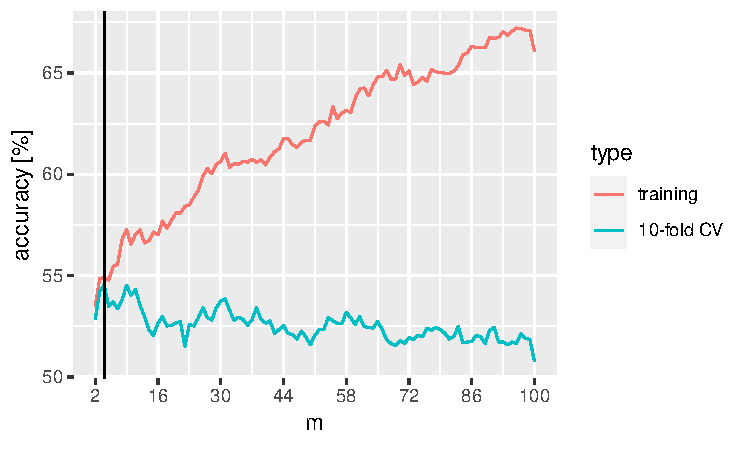
\includegraphics[width=0.8\textwidth]{log_acc_vs_m.pdf}
  \caption{Training and 10-fold CV accuracy for the logistic regression as a function of the length $m$ of the moving window. The vertical black line indicates the value of $m=4$ for which the 10-fold CV accuracy of the logistic regression fit is maximized.}
  \label{fig:log_acc_vs_m}
\end{figure}

\begin{figure}[h!]
  \centering
  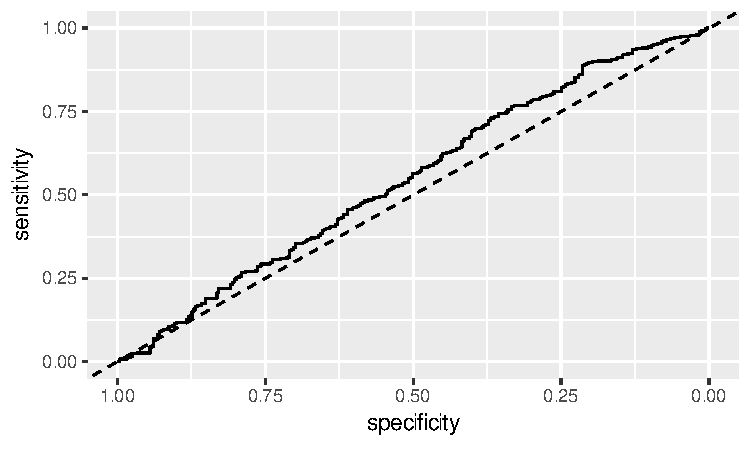
\includegraphics[width=0.8\textwidth]{log_roc.pdf}
  \caption{ROC curve of the logistic regression fit. The dashed diagonal line is the ROC curve of a random classifier. For the logistic regression fit, the AUC is $12$.}
  \label{fig:log_roc}
\end{figure}

The confusion matrix of the logistic regression w.r.t. the test set is reported in Tab.~\ref{tab:log_conf_mat}. As already observed in the ROC curve, the logistic regression fit predicts both increasing and decreasing Bitcoin market prices. This impression is also quantified by the sensitivity and specificity reported in Tab.~\ref{tab:log_results}. Even the test accuracy of the logistic regression fit is larger than the one of the majority predictor.

\begin{table}
\centering
\begin{tabular}{c|c|c}
  \backslashbox{predicted}{true} & $0$ & $1$ \\
 \hline
 $0$ & $77$ & $73$ \\  
 \hline
 $1$ & $232$ & $313$    
\end{tabular}
 \caption{Confusion matrix of the logistic regression fit on the test set.}
 \label{tab:log_conf_mat}
\end{table}

\begin{table}[h!]
\centering
\begin{tabular}{c|c|c}
accuracy [\%] & sensitivity [\%] & specificity [\%] \\
   \hline
$56.70$ & $81.09$ & $24.92$
\end{tabular}
 \caption{Accuracy, sensitivity, and specificity of the logistic regression fit on the test set.}
 \label{tab:log_results}
\end{table}

In Tab.~\ref{tab:log_coef} the coefficients of the logistic regression fit for the best value of $m$ are stated. Almost all of the coefficients are not significant based on their relative high standard deviation, and on the low $z$ scores close to zero. This has mainly two reasons. On the one hand, the actual relationship between the features and the label is not modeled completely by the logistic regression. On the other hand, some of the features are correlated, as can be observed when computing the so-called variance inflation coefficients (VIF) of the coefficients. In Tab.~\ref{tab:log_vif}, the square-root of the VIF coefficients for all of the coefficients are reported. It reports how much larger the standard deviation of each coefficient is compared to the case where there is no correlation between the features.

\begin{table}[h!]
\centering
\begin{tabular}{c||c|c|c|c}
coefficient & estimate & std. & $z$ score & $P(>|z|)\,[\%]$ \\
 \hline
 \hline
(intercept) & $-0.15$ & $0.22$ & $-0.688$ & $49.13$ \\  
 \hline
 market price ($t_{-2}$) & $0.45$ & $-0.60$ & $0.764$ & $44.51$\\   
 \hline
market price ($t_{-1}$) & $0.71$ & $0.82$ & $0.874$ & $38.20$\\
\hline
market price ($t_{0}$) & $-0.65$ & $0.57$ & $-1.121$ & $26.22$\\
\hline
\# transactions ($t_{-2}$) & $-0.28$ & $0.27$ & $-1.040$ & $29.81$\\
\hline
\# transactions ($t_{-1}$) & $0.20$ & $0.32$ & $0.624$ & $53.28$\\
\hline
\# transactions ($t_{0}$) & $0.11$ & $0.27$ & $0.394$ & $69.32$\\
\hline
avg. block size ($t_{-2}$) & $-0.10$ & $0.28$ & $-0.252$ & $80.10$\\
\hline
avg. block size ($t_{-1}$) & $-0.54$ & $0.32$ & $-1.682$ & $9.25$\\
\hline
avg. block size ($t_{0}$) & $0.69$ & $0.28$ & $2.501$ & $1.24$\\
\hline
hash rate ($t_{-2}$) & $-0.10$ & $0.26$ & $-0.171$ & $86.44$\\
\hline
hash rate ($t_{-1}$) & $-0.10$ & $0.28$ & $-0.043$ & $96.56$\\
\hline
hash rate ($t_{0}$) & $-0.10$ & $0.26$ & $-0.029$ & $97.67$\\
\end{tabular}
 \caption{Estimated coefficients of the logistic regression fit for a moving window length of $m=4$. For each coefficient, the standard deviation, the $z$ score, and the probability to obtain a $z$ score with an absolute value larger than the obtained one based on the $z$ statistic are given.}
 \label{tab:log_coef}
\end{table}

\begin{table}[h!]
\centering
\begin{tabular}{c|c}
coefficient & $\sqrt{VIF}$ \\
 \hline
 \hline
 market price ($t_{-2}$) & $4.69$ \\   
 \hline
market price ($t_{-1}$) & $6.64$ \\
\hline
market price ($t_{0}$) & $4.82$ \\
\hline
\# transactions ($t_{-2}$) & $1.68$ \\
\hline
\# transactions ($t_{-1}$) & $2.01$ \\
\hline
\# transactions ($t_{0}$) & $1.70$ \\
\hline
avg. block size ($t_{-2}$) & $1.78$ \\
\hline
avg. block size ($t_{-1}$) & $2.08$ \\
\hline
avg. block size ($t_{0}$) & $1.79$\\
\hline
hash rate ($t_{-2}$) & $1.45$ \\
\hline
hash rate ($t_{-1}$) & $1.55$ \\
\hline
hash rate ($t_{0}$) & $1.46$ \\
\end{tabular}
 \caption{Square-root of the VIF for all of the coefficients in the logistic regression from Tab.~\ref{tab:log_coef}.}
 \label{tab:log_vif}
\end{table}

\subsection{K-Nearest Neighbors Algorithm}
The next algorithm that is trained on the binary classification dataset is the K-nearest neighbors algorithm. The K-nearest neighbors algorithm has the hyperparameter K - the number of nearest neighbors that is considered for each prediction. Thus, for each moving window length $m$, additionally the hyperparameter $K$ is optimized via 10-fold CV. Fig.~\ref{fig:knn_acc_vs_m} shows the accuracies of the best predictor for each moving window length $m$. The highest 10-fold CV accuracy is obtained for $m=91$. 

\begin{figure}[h!]
  \centering
  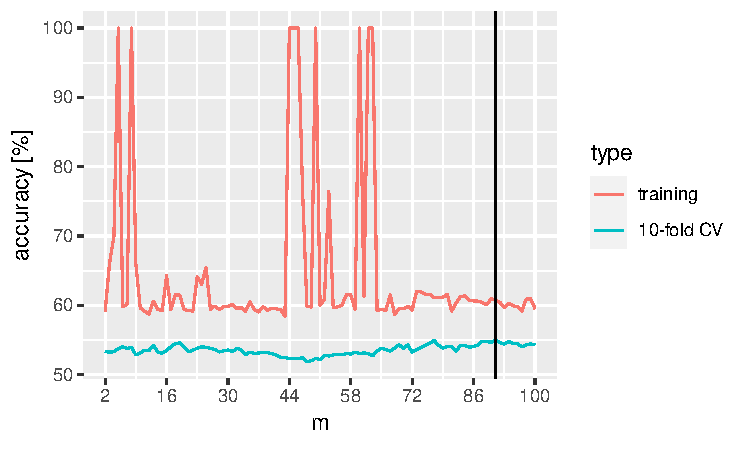
\includegraphics[width=0.8\textwidth]{knn_acc_vs_m.pdf}
  \caption{Training and 10-fold CV accuracy for the K-nearest neighbors algorithm as a function of the length $m$ of the moving window. For each $m$, the number of nearest neighbors $K$ for which the 10-fold CV accuracy is the highest is reported. The optimal value of $K_{max}$ for each moving window length $m$ is reported in Fig.~\ref The vertical black line indicates the value of $m=91$ for which the 10-fold CV accuracy of the K-nearest neighbors regression is maximized.}
  \label{fig:knn_acc_vs_m}
\end{figure}

\begin{figure}[h!]
  \centering
  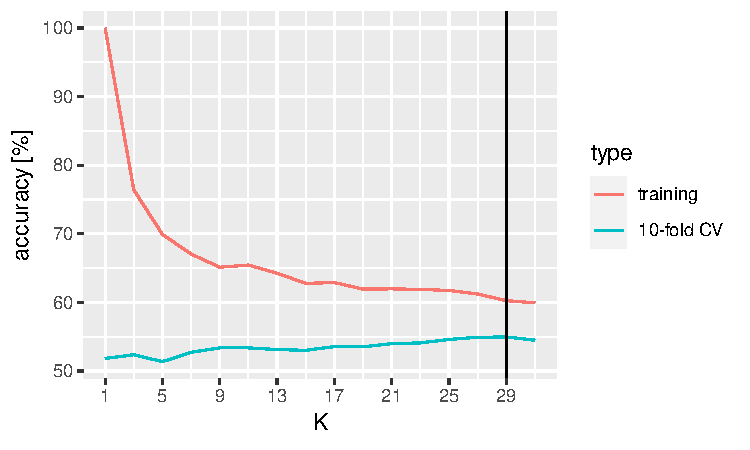
\includegraphics[width=0.8\textwidth]{knn_acc_vs_K.pdf}
  \caption{Training and 10-fold CV accuracy for the K-neareast neighbors algorithm as a functio of $K$ for the optimal moving window size $m=91$. The vertical black line indicates the value of $K_{max} = 29$ for which the 10-fold CV accuracy of the K-nearest neighbors algorithm is maximized.}
  \label{fig:knn_acc_vs_K}
\end{figure}

\begin{figure}[h!]
  \centering
  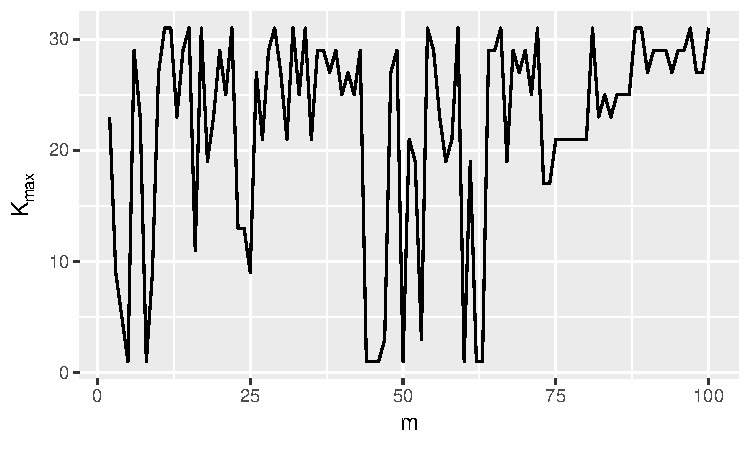
\includegraphics[width=0.8\textwidth]{knn_K_max.pdf}
  \caption{Number of nearest neighbors $K_{max}$ for which the 10-fold CV accuracy for each moving window length $m$ is maximized.}
  \label{fig:knn_K_max}
\end{figure}

\begin{figure}[h!]
  \centering
  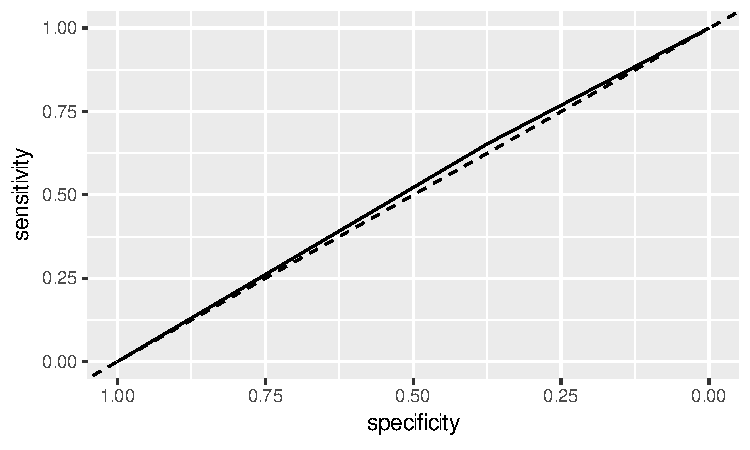
\includegraphics[width=0.8\textwidth]{knn_roc.pdf}
  \caption{ROC curve for the K-nearest neighbors algorithm. The dashed diagonal line is the ROC curve of a random classifier. For the K-neareast neighbors algorithm, the AUC is $12$.}
  \label{fig:knn_roc}
\end{figure}

\begin{table}[h!]
\centering
\begin{tabular}{c|c|c}
  \backslashbox{predicted}{true} & $0$ & $1$ \\
 \hline
 $0$ & $115$ & $133$ \\  
 \hline
 $1$ & $194$ & $253$    
\end{tabular}
 \caption{confusion matrix of knn on test set}
\end{table}

\begin{table}[h!]
\centering
\begin{tabular}{c|c|c}
accuracy [\%] & sensitivity [\%] & specificity [\%] \\
   \hline
$51.80$ & $65.54$ & $37.21$
\end{tabular}
 \caption{Accuracy, sensitivity, and specificity for the K-nearest neighbors algorithm on the test set.}
 \label{tab:knn_results}
\end{table}

\subsection{Deep Neural Network}

- sensitivity: \SI{100.00}{\percent}
- specificity: \SI{0.00}{\percent}

\begin{figure}[h!]
  \centering
  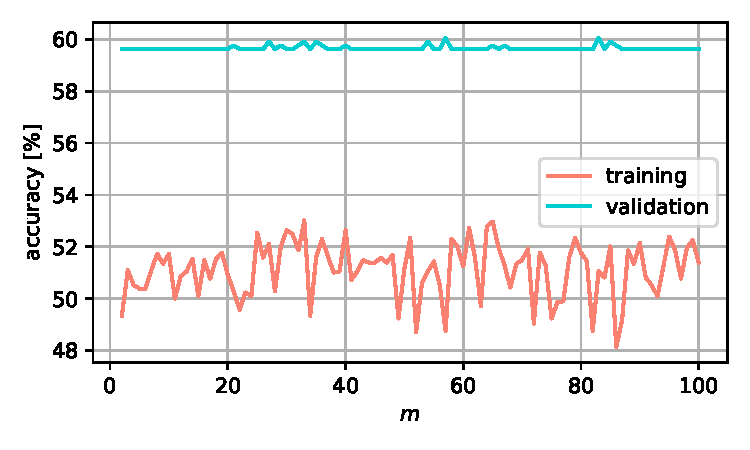
\includegraphics[width=0.8\textwidth]{dnn_acc_vs_m.pdf}
  \caption{accuracy dnn}
\end{figure}

\begin{figure}[h!]
  \centering
  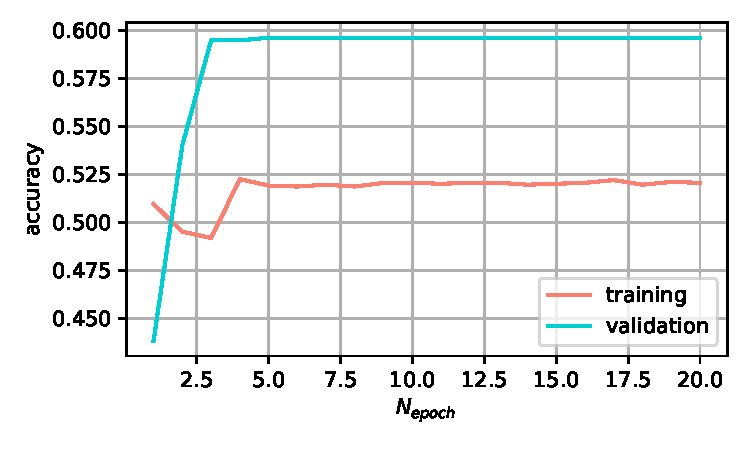
\includegraphics[width=0.8\textwidth]{dnn_acc_vs_N.pdf}
  \caption{accuracy N max dnn}
\end{figure}

\begin{figure}[h!]
  \centering
  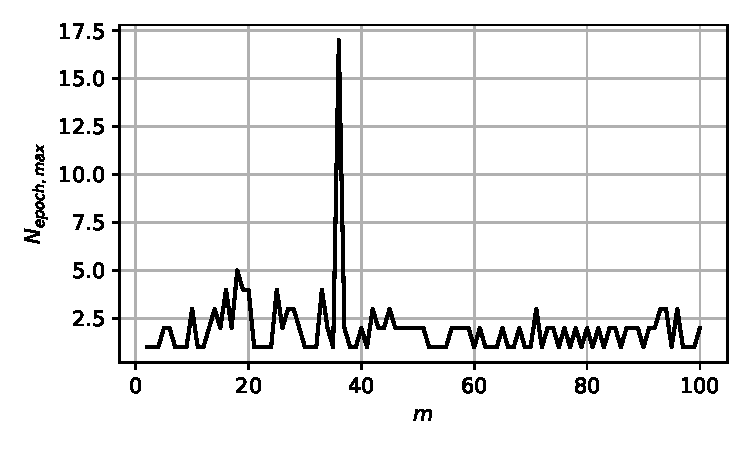
\includegraphics[width=0.8\textwidth]{dnn_N_max.pdf}
  \caption{N max dnn}
\end{figure}

\begin{table}[h!]
\centering
\begin{tabular}{c|c|c}
  \backslashbox{predicted}{true} & $0$ & $1$ \\
 \hline
 $0$ & $0$ & $0$ \\  
 \hline
 $1$ & $309$ & $386$    
\end{tabular}
 \caption{confusion matrix of dnn on test set}
\end{table}

\begin{table}[h!]
\centering
\begin{tabular}{c|c|c}
accuracy [\%] & sensitivity [\%] & specificity [\%] \\
   \hline
$55.54$ & $100.00$ & $0.00$
\end{tabular}
 \caption{Accuracy, sensitivity, and specificity of the deep neural network on the test set.}
 \label{tab:dnn_results}
\end{table}